\chapter{Strings}
\label{strings}


\section{A string is a sequence}

\index{sequence}
\index{character}
\index{bracket operator}
\index{operator!bracket}
A string is a {\bf sequence} of characters.  
You can access the characters one at a time with the
bracket operator:

\begin{verbatim}
>>> fruit = 'banana'
>>> letter = fruit[1]
\end{verbatim}
%
The second statement selects character number 1 from {\tt
fruit} and assigns it to {\tt letter}.  
\index{index}

The expression in brackets is called an {\bf index}.  
The index indicates which character in the sequence you
want (hence the name).

But you might not get what you expect:

\begin{verbatim}
>>> print letter
a
\end{verbatim}
%
For most people, the first letter of \verb"'banana'" is {\tt b}, not
{\tt a}.  But for computer scientists, the index is an offset from the
beginning of the string, and the offset of the first letter is zero.

\begin{verbatim}
>>> letter = fruit[0]
>>> print letter
b
\end{verbatim}
%
So {\tt b} is the 0th letter (``zero-eth'') of \verb"'banana'", {\tt a}
is the 1th letter (``one-eth''), and {\tt n} is the 2th (``two-eth'')
letter.
\index{index!starting at zero}
\index{zero, index starting at}

You can use any expression, including variables and operators, as an
index, but the value of the index has to be an integer.  Otherwise you
get:
\index{index}
\index{exception!TypeError}
\index{TypeError}

\begin{verbatim}
>>> letter = fruit[1.5]
TypeError: string indices must be integers, not float
\end{verbatim}
%

\section{{\tt len}}
\index{len function}
\index{function!len}

{\tt len} is a built-in function that returns the number of characters
in a string:

\begin{verbatim}
>>> fruit = 'banana'
>>> len(fruit)
6
\end{verbatim}
%
To get the last letter of a string, you might be tempted to try something
like this:
\index{exception!IndexError}
\index{IndexError}

\begin{verbatim}
>>> length = len(fruit)
>>> last = fruit[length]
IndexError: string index out of range
\end{verbatim}
%
The reason for the {\tt IndexError} is that there is no letter in {\tt
'banana'} with the index 6.  Since we started counting at zero, the
six letters are numbered 0 to 5.  To get the last character, you have
to subtract 1 from {\tt length}:

\begin{verbatim}
>>> last = fruit[length-1]
>>> print last
a
\end{verbatim}
%
Alternatively, you can use negative indices, which count backward from
the end of the string.  The expression {\tt fruit[-1]} yields the last
letter, {\tt fruit[-2]} yields the second to last, and so on.
\index{index!negative}
\index{negative index}


\section{Traversal with a {\tt for} loop}
\label{for}
\index{traversal}
\index{loop!traversal}
\index{for loop}
\index{loop!for}
\index{statement!for}
\index{traversal}

A lot of computations involve processing a string one character at a
time.  Often they start at the beginning, select each character in
turn, do something to it, and continue until the end.  This pattern of
processing is called a {\bf traversal}.  One way to write a traversal
is with a {\tt while} loop:

\begin{verbatim}
index = 0
while index < len(fruit):
    letter = fruit[index]
    print letter
    index = index + 1
\end{verbatim}
%
This loop traverses the string and displays each letter on a line by
itself.  The loop condition is {\tt index < len(fruit)}, so
when {\tt index} is equal to the length of the string, the
condition is false, and the body of the loop is not executed.  The
last character accessed is the one with the index {\tt len(fruit)-1},
which is the last character in the string.

\begin{exercise}

Write a function that takes a string as an argument
and displays the letters backward, one per line.

\end{exercise}

Another way to write a traversal is with a {\tt for} loop:

\begin{verbatim}
for char in fruit:
    print char
\end{verbatim}
%
Each time through the loop, the next character in the string is assigned
to the variable {\tt char}.  The loop continues until no characters are
left.
\index{concatenation}
\index{abecedarian}
\index{McCloskey, Robert}

The following example shows how to use concatenation (string addition)
and a {\tt for} loop to generate an abecedarian series (that is, in
alphabetical order).  In Robert McCloskey's book {\em Make
Way for Ducklings}, the names of the ducklings are Jack, Kack, Lack,
Mack, Nack, Ouack, Pack, and Quack.  This loop outputs these names in
order:

\begin{verbatim}
prefixes = 'JKLMNOPQ'
suffix = 'ack'

for letter in prefixes:
    print letter + suffix
\end{verbatim}
%
The output is:

\begin{verbatim}
Jack
Kack
Lack
Mack
Nack
Oack
Pack
Qack
\end{verbatim}
%
Of course, that's not quite right because ``Ouack'' and
``Quack'' are misspelled.

\begin{exercise}

Modify the program to fix this error.

\end{exercise}



\section{String slices}
\label{slice}
\index{slice operator}
\index{operator!slice}
\index{index!slice}
\index{string!slice}
\index{slice!string}

A segment of a string is called a {\bf slice}.  Selecting a slice is
similar to selecting a character:

\begin{verbatim}
>>> s = 'Monty Python'
>>> print s[0:5]
Monty
>>> print s[6:12]
Python
\end{verbatim}
%
The operator {\tt [n:m]} returns the part of the string from the 
``n-eth'' character to the ``m-eth'' character, including the first but
excluding the last.  This behavior is counterintuitive, but it might
help to imagine the indices pointing {\em between} the
characters, as in Figure~\ref{fig.banana}.

\begin{figure}
\centerline
{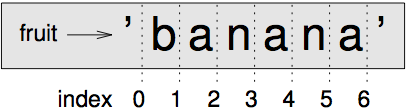
\includegraphics[scale=0.8]{figs/banana.pdf}}
\caption{Slice indices.}
\label{fig.banana}
\end{figure}


If you omit the first index (before the colon), the slice starts at
the beginning of the string.  If you omit the second index, the slice
goes to the end of the string:

\begin{verbatim}
>>> fruit = 'banana'
>>> fruit[:3]
'ban'
>>> fruit[3:]
'ana'
\end{verbatim}
%
If the first index is greater than or equal to the second the result
is an {\bf empty string}, represented by two quotation marks:
\index{quotation mark}

\begin{verbatim}
>>> fruit = 'banana'
>>> fruit[3:3]
''
\end{verbatim}
%
An empty string contains no characters and has length 0, but other
than that, it is the same as any other string.

\begin{exercise}

Given that {\tt fruit} is a string, what does
{\tt fruit[:]} mean?
\index{copy!slice}
\index{slice!copy}

\end{exercise}


\section{Strings are immutable}
\index{mutability}
\index{immutability}
\index{string!immutable}

It is tempting to use the {\tt []} operator on the left side of an
assignment, with the intention of changing a character in a string.
For example:
\index{TypeError}
\index{exception!TypeError}

\begin{verbatim}
>>> greeting = 'Hello, world!'
>>> greeting[0] = 'J'
TypeError: 'str' object does not support item assignment
\end{verbatim}
%
The ``object'' in this case is the string and the ``item'' is
the character you tried to assign.  For now, an {\bf object} is
the same thing as a value, but we will refine that definition
later.  An {\bf item} is one of the values in a sequence.
\index{object}
\index{item assignment}
\index{assignment!item}
\index{immutability}

The reason for the error is that
strings are {\bf immutable}, which means you can't change an
existing string.  The best you can do is create a new string
that is a variation on the original:

\begin{verbatim}
>>> greeting = 'Hello, world!'
>>> new_greeting = 'J' + greeting[1:]
>>> print new_greeting
Jello, world!
\end{verbatim}
%
This example concatenates a new first letter onto
a slice of {\tt greeting}.  It has no effect on
the original string.
\index{concatenation}


\section{Searching}
\label{find}

What does the following function do?
\index{find function}
\index{function!find}

\begin{verbatim}
def find(word, letter):
    index = 0
    while index < len(word):
        if word[index] == letter:
            return index
        index = index + 1
    return -1
\end{verbatim}
%
In a sense, {\tt find} is the opposite of the {\tt []} operator.
Instead of taking an index and extracting the corresponding character,
it takes a character and finds the index where that character
appears.  If the character is not found, the function returns {\tt
-1}.

This is the first example we have seen of a {\tt return} statement
inside a loop.  If {\tt word[index] == letter}, the function breaks
out of the loop and returns immediately.

If the character doesn't appear in the string, the program
exits the loop normally and  returns {\tt -1}.

This pattern of computation---traversing a sequence and returning
when we find what we are looking for---is called a {\bf search}.
\index{traversal}
\index{search pattern}
\index{pattern!search}

\begin{exercise}

Modify {\tt find} so that it has a
third parameter, the index in {\tt word} where it should start
looking.

\end{exercise}


\section{Looping and counting}
\label{counter}
\index{counter}
\index{counting and looping}
\index{looping and counting}
\index{looping!with strings}

The following program counts the number of times the letter {\tt a}
appears in a string:

\begin{verbatim}
word = 'banana'
count = 0
for letter in word:
    if letter == 'a':
        count = count + 1
print count
\end{verbatim}
%
This program demonstrates another pattern of computation called a {\bf
counter}.  The variable {\tt count} is initialized to 0 and then
incremented each time an {\tt a} is found.
When the loop exits, {\tt count}
contains the result---the total number of {\tt a}'s.

\begin{exercise}
\index{encapsulation}

Encapsulate this code in a function named {\tt
count}, and generalize it so that it accepts the string and the
letter as arguments.
\end{exercise}

\begin{exercise}

Rewrite this function so that instead of
traversing the string, it uses the three-parameter version of {\tt
find} from the previous section.

\end{exercise}


\section{String methods}

A {\bf method} is similar to a function---it takes arguments and
returns a value---but the syntax is different.  For example, the
method {\tt upper} takes a string and returns a new string with
all uppercase letters:
\index{method}
\index{string!method}

Instead of the function syntax {\tt upper(word)}, it uses
the method syntax {\tt word.upper()}.
\index{dot notation}

\begin{verbatim}
>>> word = 'banana'
>>> new_word = word.upper()
>>> print new_word
BANANA
\end{verbatim}
%
This form of dot notation specifies the name of the method, {\tt
upper}, and the name of the string to apply the method to, {\tt
word}.  The empty parentheses indicate that this method takes no
argument.
\index{parentheses!empty}

A method call is called an {\bf invocation}; in this case, we would
say that we are invoking {\tt upper} on the {\tt word}.
\index{invocation}

As it turns out, there is a string method named {\tt find} that
is remarkably similar to the function we wrote:

\begin{verbatim}
>>> word = 'banana'
>>> index = word.find('a')
>>> print index
1
\end{verbatim}
%
In this example, we invoke {\tt find} on {\tt word} and pass
the letter we are looking for as a parameter.

Actually, the {\tt find} method is more general than our function;
it can find substrings, not just characters:

\begin{verbatim}
>>> word.find('na')
2
\end{verbatim}
%
It can take as a second argument the index where it should start:
\index{optional argument}
\index{argument!optional}

\begin{verbatim}
>>> word.find('na', 3)
4
\end{verbatim}
%
And as a third argument the index where it should stop:

\begin{verbatim}
>>> name = 'bob'
>>> name.find('b', 1, 2)
-1
\end{verbatim}
%
This search fails because {\tt b} does not
appear in the index range from {\tt 1} to {\tt 2} (not including {\tt
2}).


\begin{exercise}
\index{count method}
\index{method!count}

There is a string method called {\tt count} that is similar
to the function in the previous exercise.  Read the documentation
of this method
and write an invocation that counts the number of {\tt a}s
in \verb"'banana'".
\end{exercise}


\begin{exercise}
\index{string method}
\index{method!string}

Read the documentation of the string methods at
\url{http://docs.python.org/2/library/stdtypes.html#string-methods}.
You might want to experiment with some of them to make sure you
understand how they work.  {\tt strip} and {\tt replace} are
particularly useful.

The documentation uses a syntax that might be confusing.
For example, in \verb"find(sub[, start[, end]])", the brackets
indicate optional arguments.  So {\tt sub} is required, but
{\tt start} is optional, and if you include {\tt start},
then {\tt end} is optional.
\end{exercise}


\section{The {\tt in} operator}
\label{inboth}
\index{in operator}
\index{operator!in}
\index{boolean operator}
\index{operator!boolean}

The word {\tt in} is a boolean operator that takes two strings and
returns {\tt True} if the first appears as a substring in the second:

\begin{verbatim}
>>> 'a' in 'banana'
True
>>> 'seed' in 'banana'
False
\end{verbatim}
%
For example, the following function prints all the
letters from {\tt word1} that also appear in {\tt word2}:

\begin{verbatim}
def in_both(word1, word2):
    for letter in word1:
        if letter in word2:
            print letter
\end{verbatim}
%
With well-chosen variable names,
Python sometimes reads like English.  You could read
this loop, ``for (each) letter in (the first) word, if (the) letter 
(appears) in (the second) word, print (the) letter.''

Here's what you get if you compare apples and oranges:

\begin{verbatim}
>>> in_both('apples', 'oranges')
a
e
s
\end{verbatim}
%

\section{String comparison}
\index{string!comparison}
\index{comparison!string}

The relational operators work on strings.  To see if two strings are equal:

\begin{verbatim}
if word == 'banana':
    print 'All right, bananas.'
\end{verbatim}
%
Other relational operations are useful for putting words in alphabetical
order:

\begin{verbatim}
if word < 'banana':
    print 'Your word,' + word + ', comes before banana.'
elif word > 'banana':
    print 'Your word,' + word + ', comes after banana.'
else:
    print 'All right, bananas.'
\end{verbatim}
%
Python does not handle uppercase and lowercase letters the same way
that people do.  All the uppercase letters come before all the
lowercase letters, so:

\begin{verbatim}
Your word, Pineapple, comes before banana.
\end{verbatim}
%
A common way to address this problem is to convert strings to a
standard format, such as all lowercase, before performing the
comparison.  Keep that in mind in case you have to defend yourself
against a man armed with a Pineapple.


\section{Debugging}
\index{debugging}
\index{traversal}

When you use indices to traverse the values in a sequence,
it is tricky to get the beginning and end of the traversal
right.  Here is a function that is supposed to compare two
words and return {\tt True} if one of the words is the reverse
of the other, but it contains two errors:

\begin{verbatim}
def is_reverse(word1, word2):
    if len(word1) != len(word2):
        return False
    
    i = 0
    j = len(word2)

    while j > 0:
        if word1[i] != word2[j]:
            return False
        i = i+1
        j = j-1

    return True
\end{verbatim}
%
The first {\tt if} statement checks whether the words are the
same length.  If not, we can return {\tt False} immediately
and then, for the rest of the function, we can assume that the words
are the same length.  This is an example of the guardian pattern
in Section~\ref{guardian}.
\index{guardian pattern}
\index{pattern!guardian}
\index{index}

{\tt i} and {\tt j} are indices: {\tt i} traverses {\tt word1}
forward while {\tt j} traverses {\tt word2} backward.  If we find
two letters that don't match, we can return {\tt False} immediately.
If we get through the whole loop and all the letters match, we
return {\tt True}.

If we test this function with the words ``pots'' and ``stop'', we
expect the return value {\tt True}, but we get an IndexError:
\index{IndexError}
\index{exception!IndexError}

\begin{verbatim}
>>> is_reverse('pots', 'stop')
...
  File "reverse.py", line 15, in is_reverse
    if word1[i] != word2[j]:
IndexError: string index out of range
\end{verbatim}
%
For debugging this kind of error, my first move is to
print the values of the indices immediately before the line
where the error appears.

\begin{verbatim}
    while j > 0:
        print i, j        # print here
        
        if word1[i] != word2[j]:
            return False
        i = i+1
        j = j-1
\end{verbatim}
%
Now when I run the program again, I get more information:

\begin{verbatim}
>>> is_reverse('pots', 'stop')
0 4
...
IndexError: string index out of range
\end{verbatim}
%
The first time through the loop, the value of {\tt j} is 4,
which is out of range for the string \verb"'pots'".
The index of the last character is 3, so the
initial value for {\tt j} should be {\tt len(word2)-1}.
\index{semantic error}
\index{error!semantic}

If I fix that error and run the program again, I get:

\begin{verbatim}
>>> is_reverse('pots', 'stop')
0 3
1 2
2 1
True
\end{verbatim}
%
This time we get the right answer, but it looks like the loop only ran
three times, which is suspicious.  To get a better idea of what is
happening, it is useful to draw a state diagram.  During the first
iteration, the frame for \verb"is_reverse" is shows in Figure~\ref{fig.state4}.
\index{state diagram}
\index{diagram!state}

\begin{figure}
\centerline
{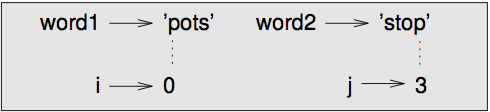
\includegraphics[scale=0.8]{figs/state4.pdf}}
\caption{State diagram.}
\label{fig.state4}
\end{figure}


I took a little license by arranging the variables in the frame
and adding dotted lines to show that the values of {\tt i} and
{\tt j} indicate characters in {\tt word1} and {\tt word2}.

\begin{exercise}
\label{isreverse}

Starting with this diagram, execute the program on paper, changing the
values of {\tt i} and {\tt j} during each iteration.  Find and fix the
second error in this function.

\end{exercise}



\section{Glossary}

\begin{description}

\item[object:] Something a variable can refer to.  For now,
you can use ``object'' and ``value'' interchangeably.
\index{object}

\item[sequence:] An ordered set; that is, a set of
values where each value is identified by an integer index.
\index{sequence}

\item[item:] One of the values in a sequence.
\index{item}

\item[index:] An integer value used to select an item in
a sequence, such as a character in a string.
\index{index}

\item[slice:] A part of a string specified by a range of indices.
\index{slice}

\item[empty string:] A string with no characters and length 0, represented
by two quotation marks.
\index{empty string}

\item[immutable:] The property of a sequence whose items cannot
be assigned.
\index{immutability}

\item[traverse:] To iterate through the items in a sequence,
performing a similar operation on each.
\index{traversal}

\item[search:] A pattern of traversal that stops
when it finds what it is looking for.
\index{search pattern}
\index{pattern!search}

\item[counter:] A variable used to count something, usually initialized
to zero and then incremented.
\index{counter}

\item[method:] A function that is associated with an object and called
using dot notation.
\index{method}

\item[invocation:] A statement that calls a method.
\index{invocation}

\end{description}


\section{Exercises}

\begin{exercise}
\index{step size}
\index{slice operator}
\index{operator!slice}

A string slice can take a third index that specifies the ``step
size;'' that is, the number of spaces between successive characters.
A step size of 2 means every other character; 3 means every third,
etc.

\begin{verbatim}
>>> fruit = 'banana'
>>> fruit[0:5:2]
'bnn'
\end{verbatim}

A step size of -1 goes through the word backwards, so
the slice \verb"[::-1]" generates a reversed string.
\index{palindrome}

Use this idiom to write a one-line version of \verb"is_palindrome"
from Exercise~\ref{palindrome}.
\end{exercise}


\begin{exercise}

The following functions are all {\em intended} to check whether a
string contains any lowercase letters, but at least some of them are
wrong.  For each function, describe what the function actually does
(assuming that the parameter is a string).

\begin{verbatim}
def any_lowercase1(s):
    for c in s:
        if c.islower():
            return True
        else:
            return False

def any_lowercase2(s):
    for c in s:
        if 'c'.islower():
            return 'True'
        else:
            return 'False'

def any_lowercase3(s):
    for c in s:
        flag = c.islower()
    return flag

def any_lowercase4(s):
    flag = False
    for c in s:
        flag = flag or c.islower()
    return flag

def any_lowercase5(s):
    for c in s:
        if not c.islower():
            return False
    return True
\end{verbatim}

\end{exercise}


\begin{exercise}
\index{letter rotation}
\index{rotation, letter}

\label{exrotate}
ROT13 is a weak form of encryption that involves ``rotating'' each
letter in a word by 13 places.  To rotate a letter means
to shift it through the alphabet, wrapping around to the beginning if
necessary, so 'A' shifted by 3 is 'D' and 'Z' shifted by 1 is 'A'.

Write a function called \verb"rotate_word"
that takes a string and an integer as parameters, and that returns
a new string that contains the letters from the original string
``rotated'' by the given amount.  

For example, ``cheer'' rotated by 7 is ``jolly'' and ``melon'' rotated
by -10 is ``cubed''.  

%For example ``sleep''
%rotated by 9 is ``bunny'' and ``latex'' rotated by 7 is ``shale''.

You might want to use the built-in functions {\tt ord}, which converts
a character to a numeric code, and {\tt chr}, which converts numeric
codes to characters.

Potentially offensive jokes on the Internet are sometimes encoded
in ROT13.  If you are not easily offended, find and decode some
of them.  Solution: \url{http://thinkpython.com/code/rotate.py}.

\end{exercise}



\section{Reading word lists}
\label{wordlist}

For the exercises in this chapter we need a list of English words.
There are lots of word lists available on the Web, but the one most
suitable for our purpose is one of the word lists collected and
contributed to the public domain by Grady Ward as part of the Moby
lexicon project (see \url{http://wikipedia.org/wiki/Moby_Project}).  It
is a list of 113,809 official crosswords; that is, words that are
considered valid in crossword puzzles and other word games.  In the
Moby collection, the filename is {\tt 113809of.fic}; you can download
a copy, with the simpler name {\tt words.txt}, from
\url{http://thinkpython.com/code/words.txt}.
\index{Moby Project}
\index{crosswords}

This file is in plain text, so you can open it with a text
editor, but you can also read it from Python.  The built-in
function {\tt open} takes the name of the file as a parameter
and returns a {\bf file object} you can use to read the file.
\index{open function}
\index{function!open}
\index{plain text}
\index{text!plain}
\index{object!file}
\index{file object}

\begin{verbatim}
>>> fin = open('words.txt')
>>> print fin
<open file 'words.txt', mode 'r' at 0xb7f4b380>
\end{verbatim}
%
{\tt fin} is a common name for a file object used for
input.  Mode \verb"'r'" indicates that this file is open for
reading (as opposed to \verb"'w'" for writing).
\index{readline method}
\index{method!readline}

The file object provides several methods for reading, including
{\tt readline}, which reads characters from the file
until it gets to a newline and returns the result as a
string:

\begin{verbatim}
>>> fin.readline()
'aa\r\n'
\end{verbatim}
%
The first word in this particular list is ``aa,'' which is a kind of
lava.  The sequence \verb"\r\n" represents two whitespace characters,
a carriage return and a newline, that separate this word from the
next.

The file object keeps track of where it is in the file, so
if you call {\tt readline} again, you get the next word:

\begin{verbatim}
>>> fin.readline()
'aah\r\n'
\end{verbatim}
%
The next word is ``aah,'' which is a perfectly legitimate
word, so stop looking at me like that.
Or, if it's the whitespace that's bothering you,
we can get rid of it with the string method {\tt strip}:
\index{strip method}
\index{method!strip}

\begin{verbatim}
>>> line = fin.readline()
>>> word = line.strip()
>>> print word
aahed
\end{verbatim}
%
You can also use a file object as part of a {\tt for} loop.
This program reads {\tt words.txt} and prints each word, one
per line:
\index{open function}
\index{function!open}

\begin{verbatim}
fin = open('words.txt')
for line in fin:
    word = line.strip()
    print word
\end{verbatim}
%

\begin{exercise}

Write a program that reads {\tt words.txt} and prints only the
words with more than 20 characters (not counting whitespace).
\index{whitespace}

\end{exercise}


\section{Exercises}

There are solutions to these exercises in the next section.
You should at least attempt each one before you read the solutions.

\begin{exercise}

In 1939 Ernest Vincent Wright published a 50,000 word novel called
{\em Gadsby} that does not contain the letter ``e.''  Since ``e'' is
the most common letter in English, that's not easy to do.

In fact, it is difficult to construct a solitary thought without using
that most common symbol.  It is slow going at first, but with caution
and hours of training you can gradually gain facility.

All right, I'll stop now.

Write a function called \verb"has_no_e" that returns {\tt True} if
the given word doesn't have the letter ``e'' in it.

Modify your program from the previous section to print only the words
that have no ``e'' and compute the percentage of the words in the list
have no ``e.''
\index{lipogram}

\end{exercise}


\begin{exercise} 

Write a function named {\tt avoids}
that takes a word and a string of forbidden letters, and
that returns {\tt True} if the word doesn't use any of the forbidden
letters.

Modify your program to prompt the user to enter a string
of forbidden letters and then print the number of words that
don't contain any of them.
Can you find a combination of 5 forbidden letters that
excludes the smallest number of words?

\end{exercise}



\begin{exercise}

Write a function named \verb"uses_only" that takes a word and a
string of letters, and that returns {\tt True} if the word contains
only letters in the list.  Can you make a sentence using only the
letters {\tt acefhlo}?  Other than ``Hoe alfalfa?''

\end{exercise}


\begin{exercise} 

Write a function named \verb"uses_all" that takes a word and a
string of required letters, and that returns {\tt True} if the word
uses all the required letters at least once.  How many words are there
that use all the vowels {\tt aeiou}?  How about {\tt aeiouy}?

\end{exercise}


\begin{exercise}

Write a function called \verb"is_abecedarian" that returns
{\tt True} if the letters in a word appear in alphabetical order
(double letters are ok).  
How many abecedarian words are there?

\index{abecedarian}

\end{exercise}


%\begin{exercise}
%\label{palindrome}
%A palindrome is a word that reads the same
%forward and backward, like ``rotator'' and ``noon.''
%Write a boolean function named \verb"is_palindrome" that
%takes a string as a parameter and returns {\tt True} if it is
%a palindrome.

%Modify your program from the previous section to print all
%of the palindromes in the word list and then print the total
%number of palindromes.
%\end{exercise}



\section{Search}
\index{search pattern}
\index{pattern!search}

All of the exercises in the previous section have something
in common; they can be solved with the search pattern we saw
in Section~\ref{find}.  The simplest example is:

\begin{verbatim}
def has_no_e(word):
    for letter in word:
        if letter == 'e':
            return False
    return True
\end{verbatim}
%
The {\tt for} loop traverses the characters in {\tt word}.  If we find
the letter ``e'', we can immediately return {\tt False}; otherwise we
have to go to the next letter.  If we exit the loop normally, that
means we didn't find an ``e'', so we return {\tt True}.
\index{traversal}

% Removing this because we haven't seen the in operator yet.
%\index{in operator}
%\index{operator!in}

%You could write this function more concisely using the {\tt in}
%operator, but I started with this version because it 
%demonstrates the logic of the search pattern.
\index{generalization}

{\tt avoids} is a more general version of \verb"has_no_e" but it
has the same structure:

\begin{verbatim}
def avoids(word, forbidden):
    for letter in word:
        if letter in forbidden:
            return False
    return True
\end{verbatim}
%
We can return {\tt False} as soon as we find a forbidden letter;
if we get to the end of the loop, we return {\tt True}.

\verb"uses_only" is similar except that the sense of the condition
is reversed:

\begin{verbatim}
def uses_only(word, available):
    for letter in word: 
        if letter not in available:
            return False
    return True
\end{verbatim}
%
Instead of a list of forbidden letters, we have a list of available
letters.  If we find a letter in {\tt word} that is not in
{\tt available}, we can return {\tt False}.

\verb"uses_all" is similar except that we reverse the role
of the word and the string of letters:

\begin{verbatim}
def uses_all(word, required):
    for letter in required: 
        if letter not in word:
            return False
    return True
\end{verbatim}
%
Instead of traversing the letters in {\tt word}, the loop
traverses the required letters.  If any of the required letters
do not appear in the word, we can return {\tt False}.
\index{traversal}

If you were really thinking like a computer scientist, you would
have recognized that \verb"uses_all" was an instance of a
previously-solved problem, and you would have written:

\begin{verbatim}
def uses_all(word, required):
    return uses_only(required, word)
\end{verbatim}
%
This is an example of a program development method called {\bf problem
recognition}, which means that you recognize the problem you are
working on as an instance of a previously-solved problem, and apply a
previously-developed solution.
\index{problem recognition}
\index{development plan!problem recognition}


\section{Looping with indices}
\index{looping!with indices}
\index{index!looping with}

I wrote the functions in the previous section with {\tt for}
loops because I only needed the characters in the strings; I didn't
have to do anything with the indices.

For \verb"is_abecedarian" we have to compare adjacent letters,
which is a little tricky with a {\tt for} loop:

\begin{verbatim}
def is_abecedarian(word):
    previous = word[0]
    for c in word:
        if c < previous:
            return False
        previous = c
    return True
\end{verbatim}


An alternative is to
use recursion:

\begin{verbatim}
def is_abecedarian(word):
    if len(word) <= 1:
        return True
    if word[0] > word[1]:
        return False
    return is_abecedarian(word[1:])
\end{verbatim}

Another option is to use a {\tt while} loop:

\begin{verbatim}
def is_abecedarian(word):
    i = 0
    while i < len(word)-1:
        if word[i+1] < word[i]:
            return False
        i = i+1
    return True
\end{verbatim}
%
The loop starts at {\tt i=0} and ends when {\tt i=len(word)-1}.  Each
time through the loop, it compares the $i$th character (which you can
think of as the current character) to the $i+1$th character (which you
can think of as the next).

If the next character is less than (alphabetically before) the current
one, then we have discovered a break in the abecedarian trend, and
we return {\tt False}.

If we get to the end of the loop without finding a fault, then the
word passes the test.  To convince yourself that the loop ends
correctly, consider an example like \verb"'flossy'".  The
length of the word is 6, so
the last time the loop runs is when {\tt i} is 4, which is the
index of the second-to-last character.  On the last iteration,
it compares the second-to-last character to the last, which is
what we want.
\index{palindrome}

Here is a version of \verb"is_palindrome" (see
Exercise~\ref{palindrome}) that uses two indices; one starts at the
beginning and goes up; the other starts at the end and goes down.

\begin{verbatim}
def is_palindrome(word):
    i = 0
    j = len(word)-1

    while i<j:
        if word[i] != word[j]:
            return False
        i = i+1
        j = j-1

    return True
\end{verbatim}

Or, if you noticed that this is an instance of a previously-solved
problem, you might have written:

\begin{verbatim}
def is_palindrome(word):
    return is_reverse(word, word)
\end{verbatim}
\index{problem recognition}
\index{development plan!problem recognition}

Assuming you did Exercise~\ref{isreverse}.


\section{Debugging}
\index{debugging}
\index{testing!is hard}
\index{program testing}

Testing programs is hard.  The functions in this chapter are
relatively easy to test because you can check the results by hand.
Even so, it is somewhere between difficult and impossible to choose a
set of words that test for all possible errors.

Taking \verb"has_no_e" as an example, there are two obvious
cases to check: words that have an 'e' should return {\tt False};
words that don't should return {\tt True}.  You should have no
trouble coming up with one of each.

Within each case, there are some less obvious subcases.  Among the
words that have an ``e,'' you should test words with an ``e'' at the
beginning, the end, and somewhere in the middle.  You should test long
words, short words, and very short words, like the empty string.  The
empty string is an example of a {\bf special case}, which is one of
the non-obvious cases where errors often lurk.
\index{special case}

In addition to the test cases you generate, you can also test
your program with a word list like {\tt words.txt}.  By scanning
the output, you might be able to catch errors, but be careful:
you might catch one kind of error (words that should not be
included, but are) and not another (words that should be included,
but aren't).

In general, testing can help you find bugs, but it is not easy to
generate a good set of test cases, and even if you do, you can't
be sure your program is correct.
\index{testing!and absence of bugs}

According to a legendary computer scientist:

\begin{quote}
Program testing can be used to show the presence of bugs, but never to
show their absence!

--- Edsger W. Dijkstra
\end{quote}
\index{Dijkstra, Edsger}


\section{Glossary}

\begin{description}

\item[file object:] A value that represents an open file.
\index{file object}
\index{object!file}

\item[problem recognition:] A way of solving a problem by
expressing it as an instance of a previously-solved problem.
\index{problem recognition}

\item[special case:] A test case that is atypical or non-obvious
(and less likely to be handled correctly).
\index{special case}

\end{description}


\section{Exercises}

\begin{exercise}
\index{Car Talk}
\index{Puzzler}
\index{double letters}

This question is based on a Puzzler that was broadcast on the radio
program {\em Car Talk} 
(\url{http://www.cartalk.com/content/puzzlers}):

\begin{quote}
Give me a word with three consecutive double letters. I'll give you a
couple of words that almost qualify, but don't. For example, the word
committee, c-o-m-m-i-t-t-e-e. It would be great except for the `i' that
sneaks in there. Or Mississippi: M-i-s-s-i-s-s-i-p-p-i. If you could
take out those i's it would work. But there is a word that has three
consecutive pairs of letters and to the best of my knowledge this may
be the only word. Of course there are probably 500 more but I can only
think of one. What is the word?
\end{quote}

Write a program to find it.  Solution: \url{http://thinkpython.com/code/cartalk1.py}.

\end{exercise}


\begin{exercise}
Here's another {\em Car Talk}
Puzzler (\url{http://www.cartalk.com/content/puzzlers}):
\index{Car Talk}
\index{Puzzler}
\index{odometer}
\index{palindrome}

\begin{quote}
``I was driving on the highway the other day and I happened to
notice my odometer. Like most odometers, it shows six digits,
in whole miles only. So, if my car had 300,000
miles, for example, I'd see 3-0-0-0-0-0.

``Now, what I saw that day was very interesting. I noticed that the
last 4 digits were palindromic; that is, they read the same forward as
backward. For example, 5-4-4-5 is a palindrome, so my odometer
could have read 3-1-5-4-4-5.

``One mile later, the last 5 numbers were palindromic. For example, it
could have read 3-6-5-4-5-6.  One mile after that, the middle 4 out of
6 numbers were palindromic.  And you ready for this? One mile later,
all 6 were palindromic!

``The question is, what was on the odometer when I first looked?''
\end{quote}

Write a Python program that tests all the six-digit numbers and prints
any numbers that satisfy these requirements.  
Solution: \url{http://thinkpython.com/code/cartalk2.py}.

\end{exercise}


\begin{exercise}
Here's another {\em Car Talk} Puzzler you can solve with a
search (\url{http://www.cartalk.com/content/puzzlers}):
\index{Car Talk}
\index{Puzzler}
\index{palindrome}

\begin{quote}
``Recently I had a visit with my mom and we realized that
the two digits that make up my age when reversed resulted in her
age. For example, if she's 73, I'm 37. We wondered how often this has
happened over the years but we got sidetracked with other topics and
we never came up with an answer.

``When I got home I figured out that the digits of our ages have been
reversible six times so far. I also figured out that if we're lucky it
would happen again in a few years, and if we're really lucky it would
happen one more time after that. In other words, it would have
happened 8 times over all. So the question is, how old am I now?''

\end{quote}

Write a Python program that searches for solutions to this Puzzler.
Hint: you might find the string method {\tt zfill} useful.

Solution: \url{http://thinkpython.com/code/cartalk3.py}.

\end{exercise}



